\chapter{Design}
\label{chapter_Design}

Im folgenden Kapitel wird auf das Design des Systems eingegangen. Zunächst wird auf den Aufbau der Hardware eingegangen. Anschließend wird sich näher mit dem Design und dem Aufbau der einzelnen Softwareelemente befasst. Zum Ende des Kapitels gibt es einen genaueren Einblick in die Gestaltung und den Aufbau des Protokoll für die RS232 Schnittstelle.

\section{Übersicht}
\label{section_Teststand}

Das Gesamtsystem setzt sich aus drei Akteuren zusammen. Der folgenden Abschnitt gibt eine kurze Übersicht über die Hauptaufgaben der einzelnen Systeme.

\begin{itemize}

\item Mess-Server
\begin{itemize}
\item Verwaltet angeschlossene Mess-Clients.
\item Speichert alle Messdaten in einer Datenbank.
\item Ermöglicht den Fernzugriff von einem PC-Client.
\end{itemize}

\item Mess-Client
\begin{itemize}
\item Übernimmt die lokale Ansteuerung der \acp{DUT}.
\item Nimmt Messdaten auf und stellt sie zur Verfügung.
\end{itemize}

\item PC-Client
\begin{itemize}
\item Parametriert die Mess-Clients.
\item Wertet Messdaten aus und stellt sie leserlich da.
\end{itemize}

\end{itemize}


\begin{figure}[H]
\begin{center}
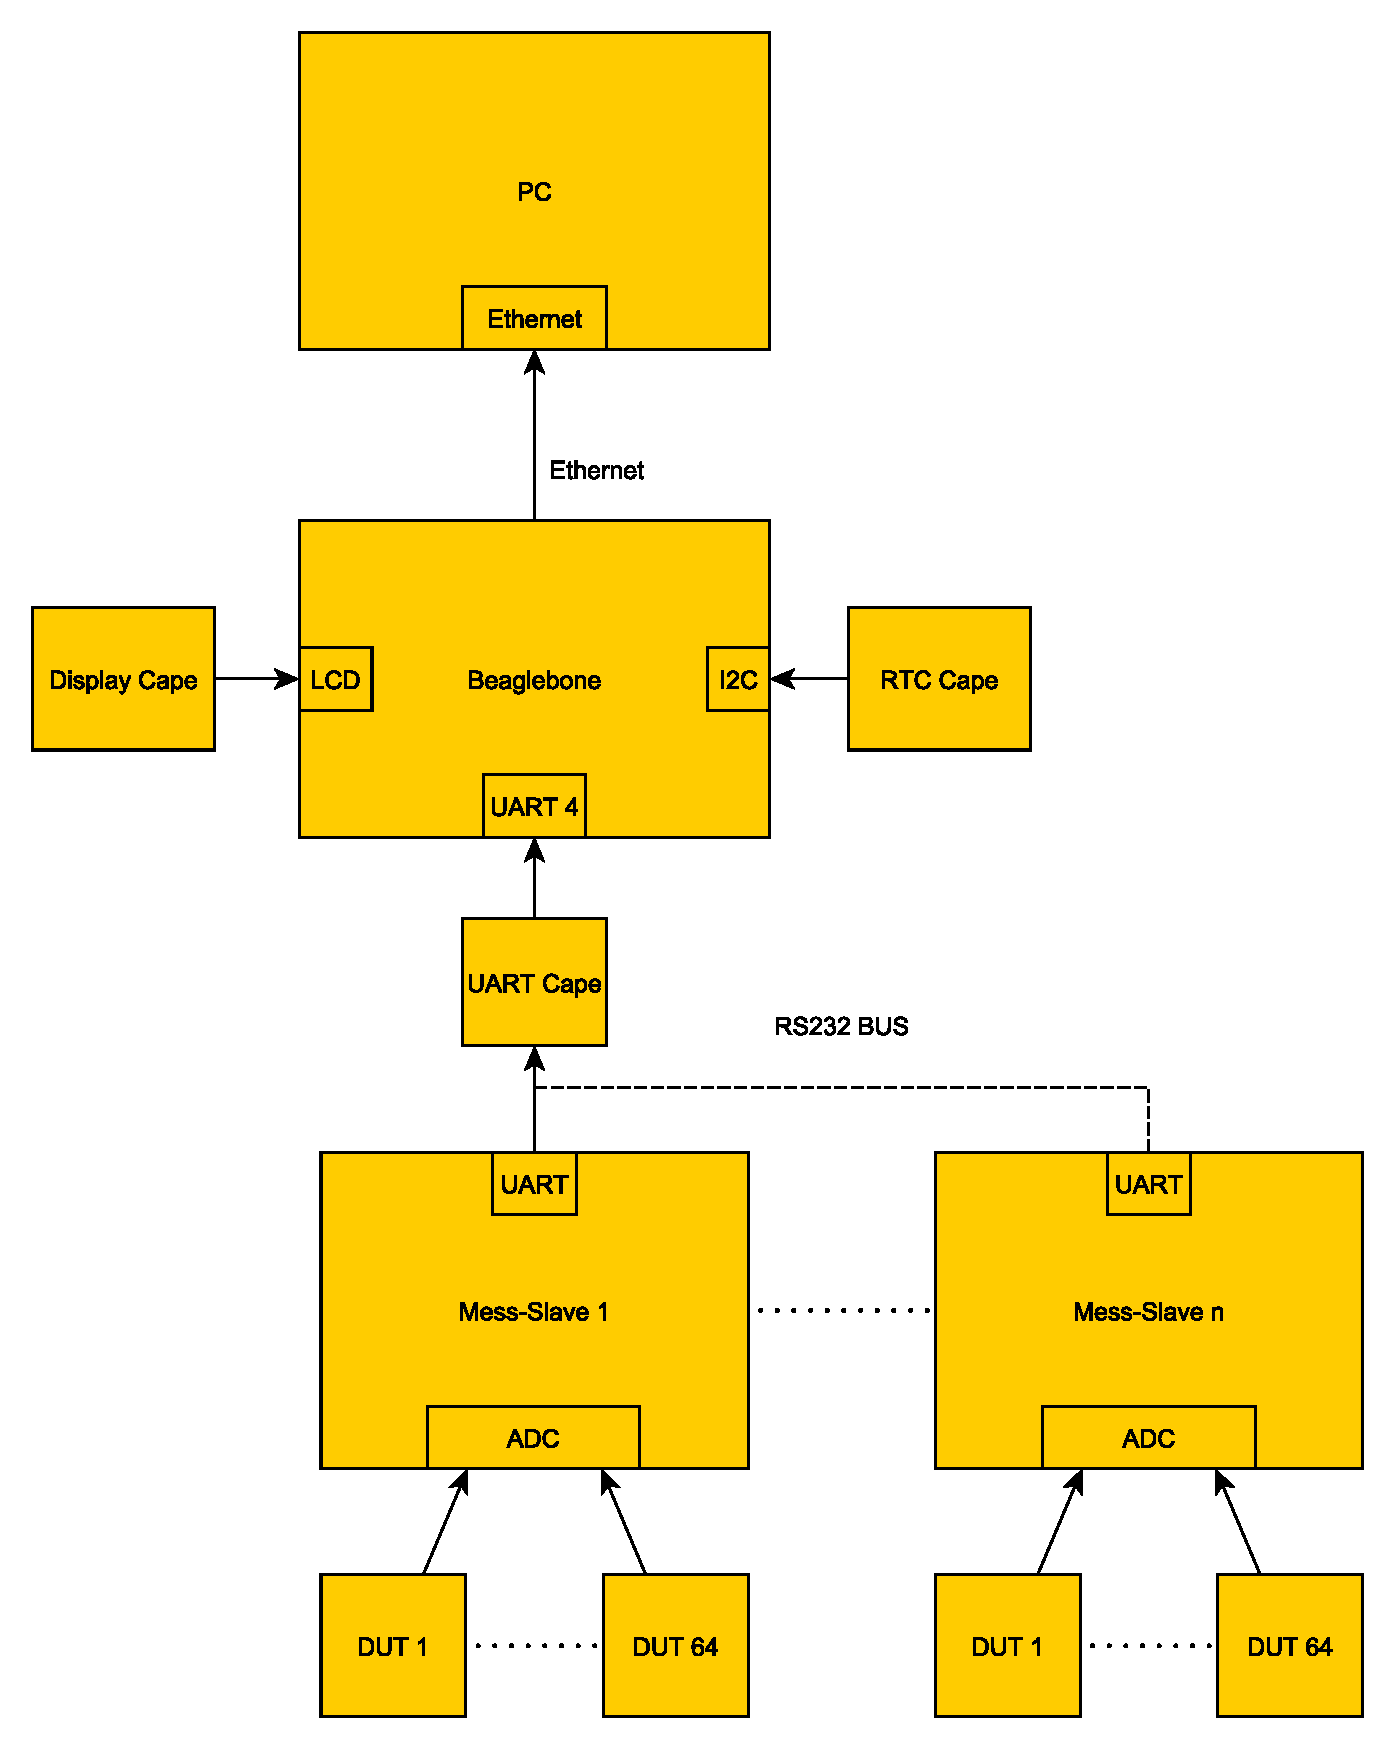
\includegraphics[width=\textwidth ]{img/general/BlockPlan.pdf}
\caption{Übersicht}
\label{figure_Übersicht}
\end{center}
\end{figure}


\section{Mess-Server}
\label{section_Mess-Server}

Als Mess-Server wird ein BeagleBone Black von Texas Instruments eingesetzt. Dabei handelt es sich um einen kostengünstigen Einplatinencomputer mit offener Hardware. Damit ist es möglich, das BeagleBone Black auf individuelle Anforderungen anzupassen und selbst herzustellen. Auch gibt es eine große Community, die ständig die Entwicklung vorantreibt.
Er arbeitet mit einem AM335x 1GHz ARM® Cortex-A8 Prozessor, verfügt über 512MB DDR3 RAM und 4GB 8-bit eMMC internen Flash Speicher. Als Spannungsversorgung dient ein 5V 2A Netzteil.


\begin{figure}[H]
\begin{center}
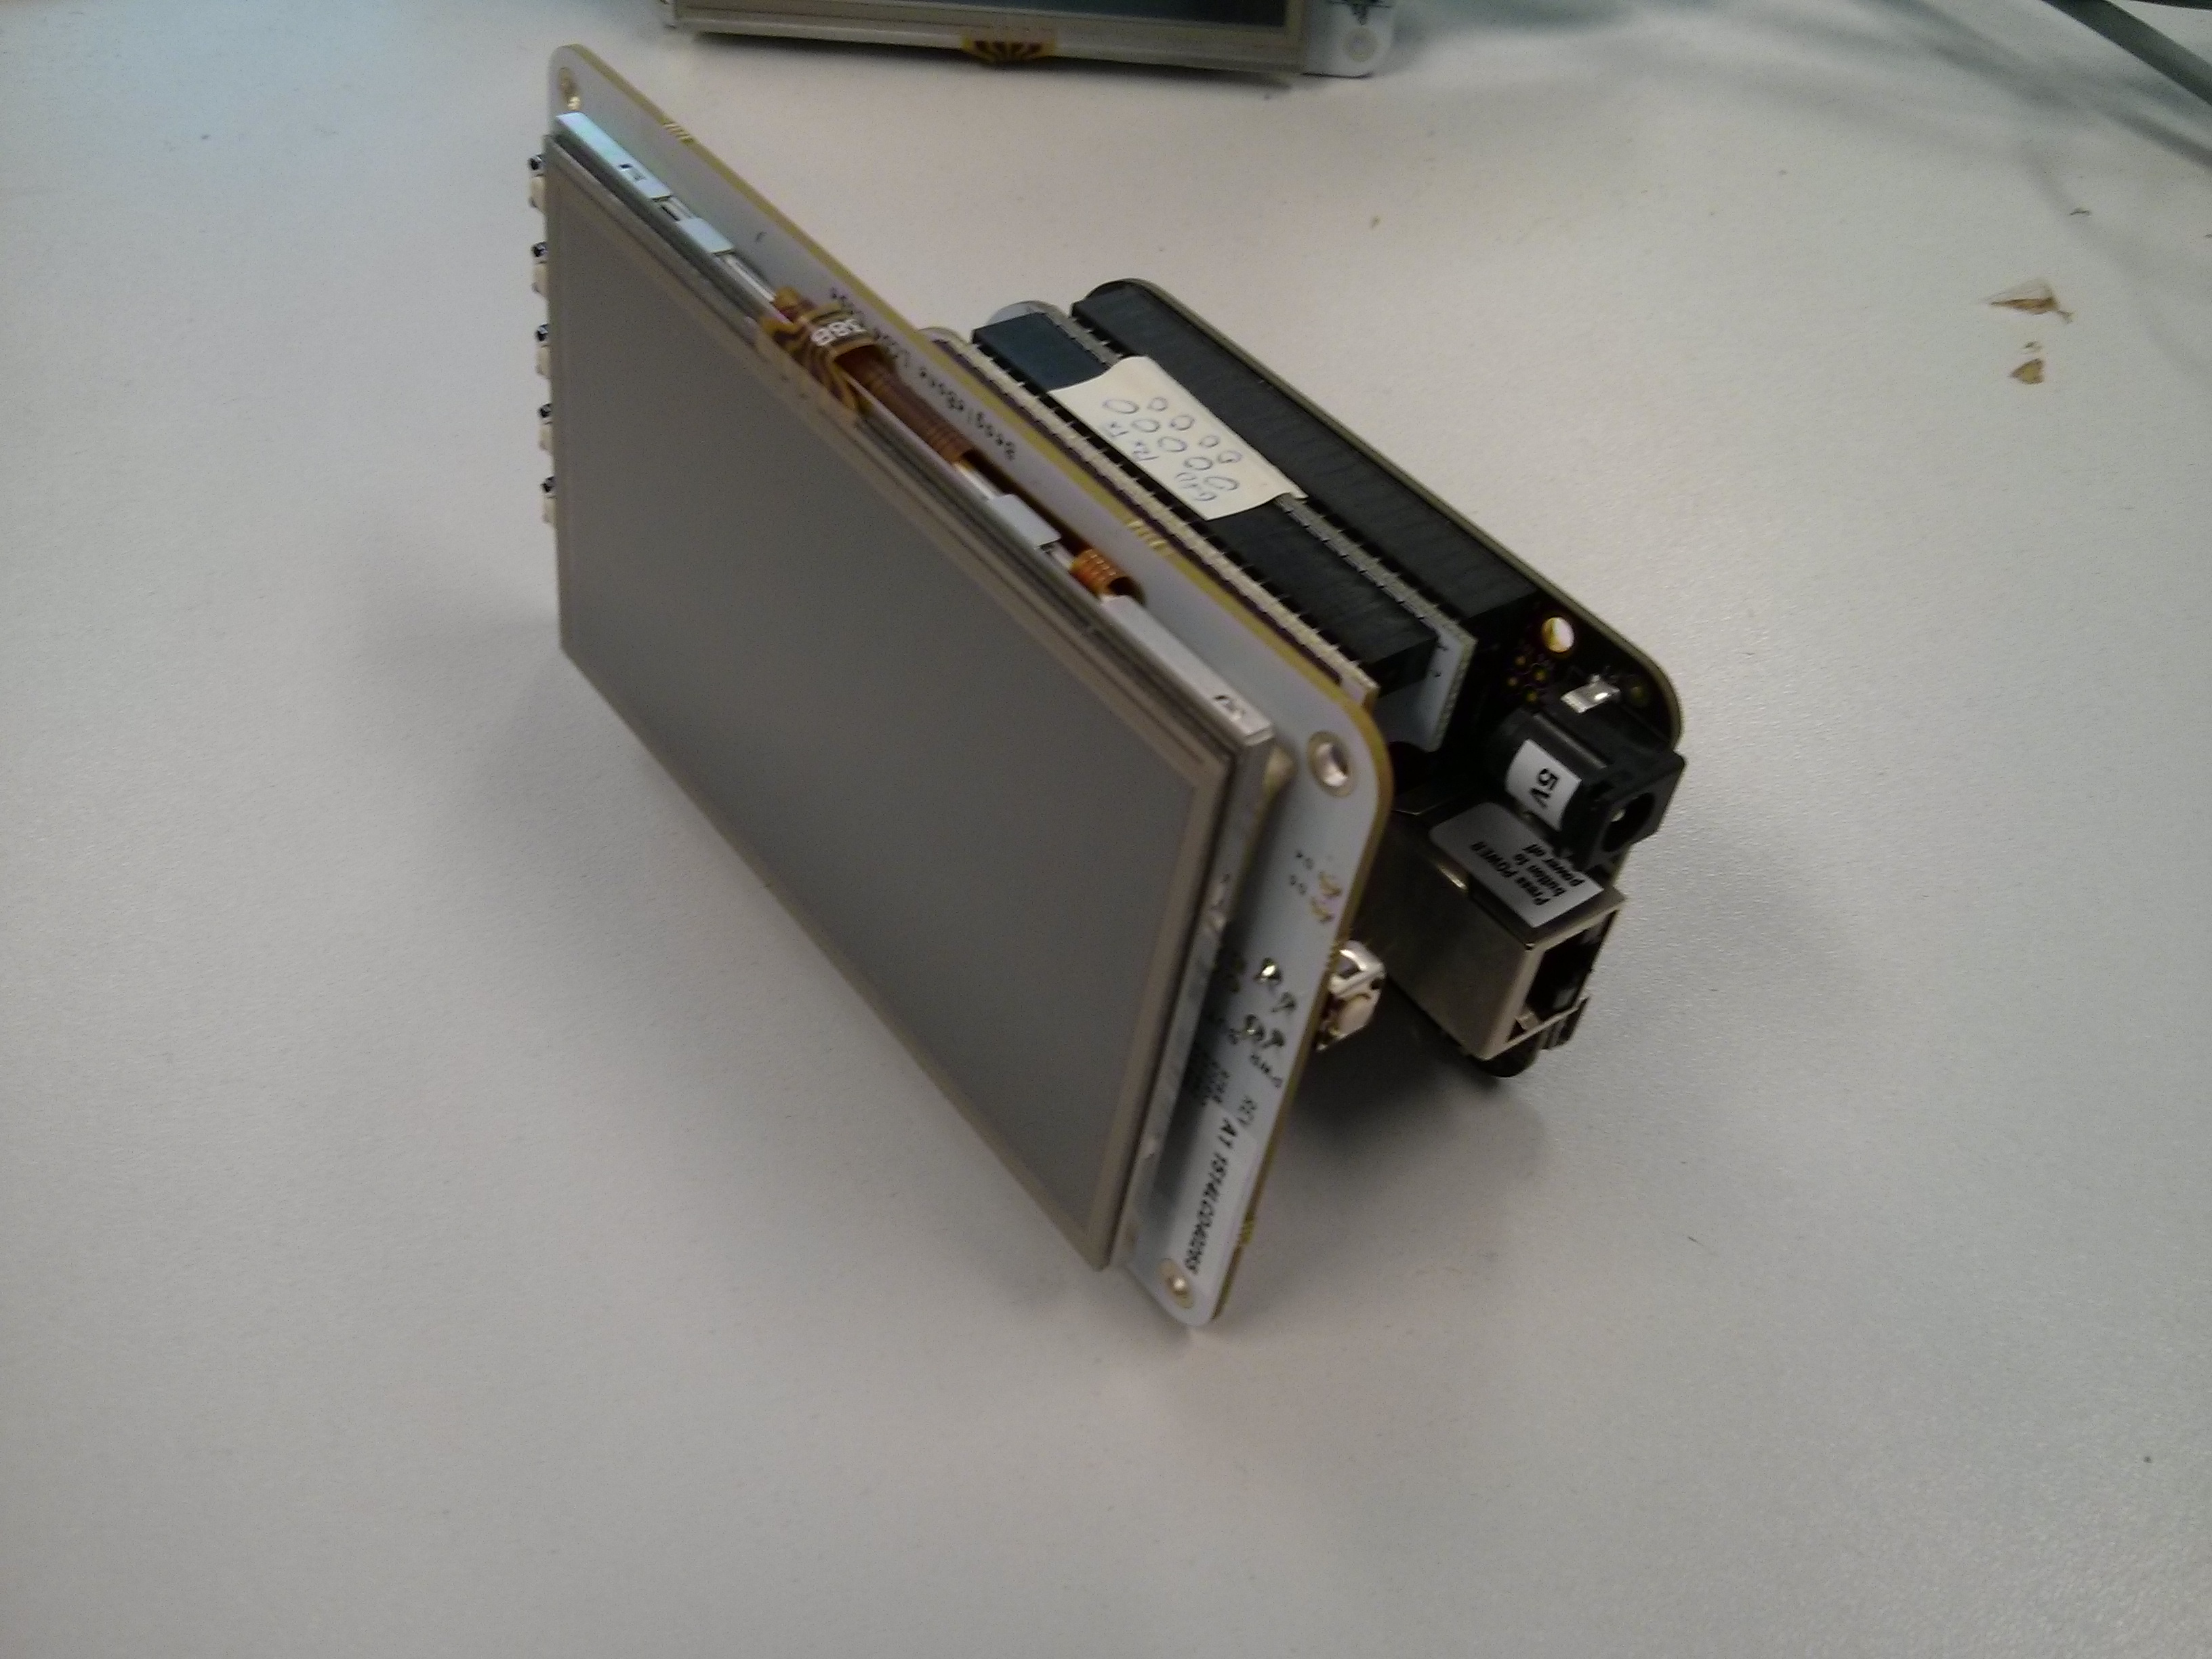
\includegraphics[width=0.8\textwidth]{img/general/BeagleBoneBlack.jpg}
\caption{BeagleBone Black}
\label{figure_Beagleboneblack}
\end{center}
\end{figure}

Trotz der Kompaktheit des BeagleBone Black, bietet er ein ausreichendes Maß an Performance. Auf ihm kommt ein Debian-GNU/Linux Betriebssystem zum Einsatz. Damit ist es möglich die umfangreichen Debian-Funktionen wie die Paketverwaltung zu nutzen. Es bietet auch den Vorteil, dass eine große Ähnlichkeit zu PC-Distributionen wie Ubuntu besteht und somit einfacher nutzbar ist (vgl. \cite{schroeder2009embedded}).\\
Außerdem sind Linux Mechanismen einfach nutzbar. So kann das RS232 Interface beispielsweise wie eine normale Datei beschrieben und gelesen werden.

\subsection{Hardware}
\label{ServerHardware}

\begin{figure}[H]
\begin{center}
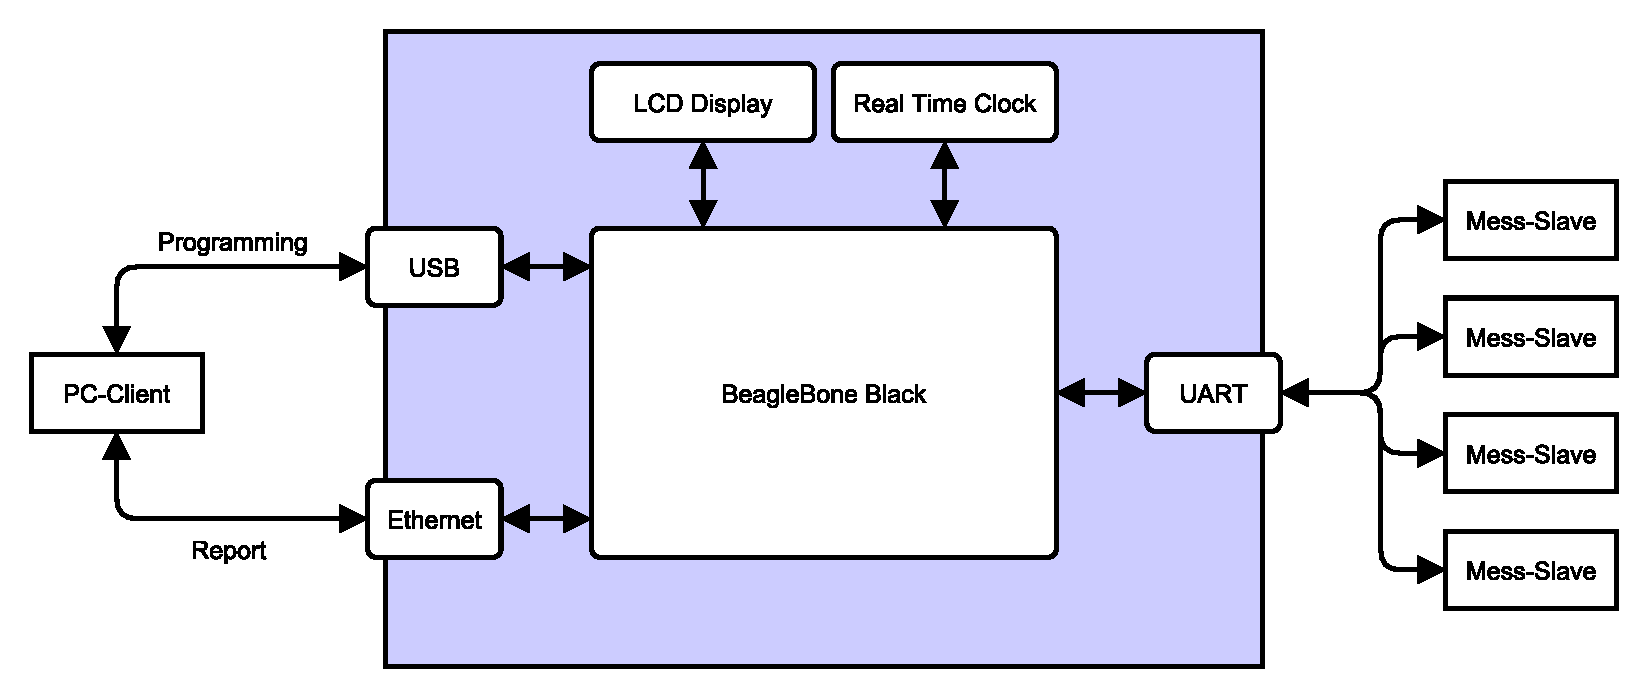
\includegraphics[width=\textwidth ]{img/general/UebersichtMaster.pdf}
\caption{Aufbau Mess-Server}
\label{figure_AufbauBleagleBone}
\end{center}
\end{figure}

Das BeagleBone selbst ist bereits sehr Leistungsstark. Um jedoch weiter Funktionen und Schnittstellen hinzuzufügen, existieren Capes. Ein Cape ist eine für das BeagleBone konzipierte Erweiterung, die direkt auf das BeagleBone aufgesteckt werden kann. Die Treiber vieler dieser Capes sind bereits in dem Betriebssystem des BeagleBones integriert oder werden vom Hersteller bereitgestellt. Somit ist die Inbetriebnahme sehr komfortable.


\textbf{ABBILDUNG EINES CAPES}


Zur Kommunikation mit den Mess-Clients wird die \ac{UART} Schnittstelle des BeagleBone Black verwendet. Dafür wird ein RS232 Cape eingesetzt. Das Cape führt die seriellen Ports UART0, UART1, UART2 und UART4 auf einen 9-poligen seriellen Stecker. Es bietet die Möglichkeit zwischen den verschiedenen Ports mittels eines Jumper auf dem Cape zu wechseln. Angeschlossen wird nach dem 3-wire Prinzip. Dabei werden lediglich Rx, Tx und die Masse verbunden. Somit ist keine Hardware-Flusssteuerung möglich.\ 

Da das BeagleBone Black kein eigenes \ac{RTC} Modul besitzt, wird auch dieses durch ein Cape hinzugefügt. Es beinhaltet eine 3V Knopfbatterie um auch im Falle einer Stromunterbrechung die aktuelle Zeit nicht zu verlieren. Dies ist sehr wichtig, da es erforderlich ist, dass das BeagleBone die aktuelle Uhrzeit und das aktuelle Datum jederzeit kennt. Denn beim Erfassen der Messdaten wird ein Zeitstempel angelegt um die Daten später zeitlich zuordnen zu können. Sollte dieser Zeitstempel nicht korrekt sein, sind die Daten bei der Auswertung nicht gültig.\ 

Um die Statusanzeige detailliert darstellen zu können, wird ein resistives LCD-Touchscreen Display eingesetzt. Es hat eine Größe von 4,3 Zoll bei einer Auflösung von 480x272 Pixeln. Dabei handelt es sich ebenso um ein Cape. Dadurch ist es möglich, das BeagleBone Black trotz den Erweiterungen kompakt zu halten. Denn die Capes sind untereinander Stapelbar.\ 


\textbf{ABBILDUNG gestapeltes BeagleBone}


Die USB Schnittstelle, welche zur Programmierung des BeagleBones verwendet wird, ist bereits vollständig einsatzbereit. Ebenso ist die Ethernet Schnittstelle, welche für den Fernzugriff auf das BeagleBone genutzt wird, bereits standardmäßig vollständig integriert.

\subsection{Software}
\label{ServerSoftware}
Die Programmierung der Software erfolgt in C++ unter Verwendung der Klassenbibliothek Qt (siehe Abschnitt \ref{section_Qt}).\\
Das Softwaredesign teilt sich in einen sequentiellen Teil für die Abfrage und Speicherung der Messwerte, sowie einen Event gesteuerten Teil für die \ac{GUI} und die externe Kommunikation für die Fernzugriffe. Die beiden Programmteile können unabhängig von einander agieren und kommunizieren ausschließlich über Signale und Slots (siehe \ref{QtSignaleSlots}). Durch diese Kapselung ist es möglich die beiden Programmteile durch andere Lösungen auszutauschen, welche lediglich die selben Signale und Slots unterstützen müssen.\ 

\subsubsection{Messdatenerfassung}
Der Hauptzyklus der Software ruft kontinuierlich die Messdaten von den Mess-Clients ab. Dafür wird ständig geprüft ob Messungen erforderlich sind. Dies geschieht durch den Vergleich der vergangenen Zeit zur letzten Messung und den gegebenen Parametern für die Messintervalle. In der Tabelle \ref{table_ParameterMessintervalle} finden sich diese Parameter.\\


\begin{table}[H]
\begin{center}
\begin{tabular}{|l|l|}\hline
Parameter & Beschreibung \\ \hline
duration\_int1 & Dauer der Zeit die Werte im 1.Interval aufgenommen werden in Tagen\\  \hline
duration\_int2 & Dauer der Zeit die Werte im 2.Interval aufgenommen werden in Tagen\\  \hline
interval\_1 & Abstand zwischen den Messungen im 1. Interval in Minuten\\  \hline
interval\_2 & Abstand zwischen den Messungen im 2. Interval in Minuten\\  \hline
interval\_3 & Abstand zwischen den Messungen nach dem 2. Interval in Minuten\\ \hline
\end{tabular}
\caption{Parameter der Messintervalle}
\label{table_ParameterMessintervalle}
\end{center}
\end{table}


Ob eine Messung erforderlich ist, lässt sich aus den gegebenen Parametern ableiten. So wird zuerst geprüft, welcher Zeitraum (\textit{duration\_int1-2}) derzeit zutrifft. Dazu wird die vergangene Zeit seit der ersten Messung mit dem Zeitraum abgeglichen. Sollten noch keine Ergebnisse vorhanden sein, ergibt dies die Erforderlichkeit einer Messung. Wenn der passende Zeitraum ausgemacht ist, wird das dazugehörige Intervall zwischen den einzelnen Messungen (\textit{interval\_1-3}) ausgemacht. Dann wird geprüft, ob die vergangene Zeit seit der letzten Messung größer ist als dieses Intervall.\ 

Anschließend wird geprüft ob der Mess-Client verfügbar ist. Dazu wird eine Namensanfrage über die RS232 Schnittstelle verschickt. Bei einer positiven Antwort wird dann eine Messung durchgeführt. Dabei werden alle \acp{ADC} der 64 möglichen \acp{DUT} mittels \textit{ADC-Value}-Befehls (siehe Tabelle \ref{table_Commands}) ausgelesen. Sobald alle 64 Werte erfolgreich ermittelt sind, werden sie in der Datenbank abgelegt. \\
Sollte keine Antwort auf die Namensanfrage erfolgen, wird in den nächsten Zyklen erneut versucht eine Verbindung zu etablieren. Bei kontinuierlich erfolglosen Verbindungsversuchen, informiert das System den Nutzer nach einer festgelegten Zeit der Abwesenheit über die Unerreichbarkeit.
 
\begin{figure}[H]
\begin{center}
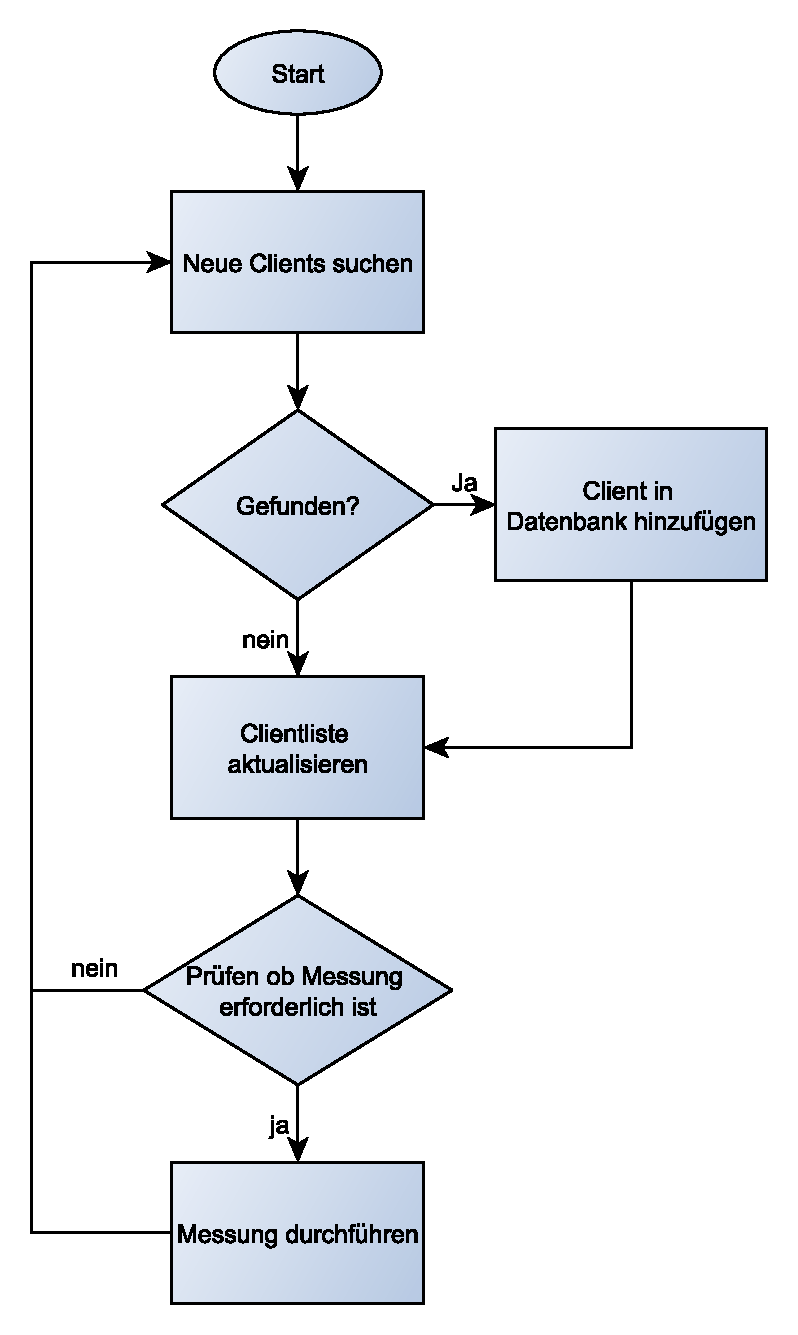
\includegraphics[width=0.5\textwidth ]{img/general/Ablaufplan_Master.pdf}
\caption{Ablaufplan}
\label{figure_Ablaufplan_Master}
\end{center}
\end{figure}
 
\newpage
\subsubsection{Benutzeroberfläche}
Um die Anforderung der Statusüberwachnung zu erfüllen, verfügt das BeagleBone über eine \ac{GUI}. Sie bietet einen einfachen Überblick über die aktuellen Vorgänge und soll auf einen Blick den Status des Mess-Servers wiedergeben.\\
Am oberen Rand der \ac{GUI} (sieht u.a. Abbildung \ref{figure_MessServerGUIStatus}) wird das aktuelle Datum und die aktuelle Uhrzeit angezeigt, sowie die derzeitige IP Adresse und der aktuelle Name. Am unteren Rand wird die derzeit ausführende Aktion in einer Statusnachricht ausgegeben.
Die \ac{GUI} ist dabei in vier Tabs unterteilt.

\textbf{Status Tab}

\begin{figure}[H]
\begin{center}
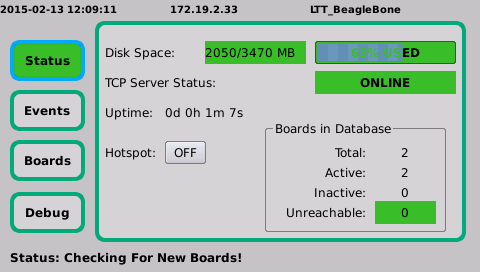
\includegraphics[width=0.5\textwidth ]{img/GUI/Server_GUI_Status1.png}
\caption{Mess-Server GUI: Status Tab}
\label{figure_MessServerGUIStatus}
\end{center}
\end{figure}

Das Erste ist das Status-Tab (siehe Abbildung \ref{figure_MessServerGUIStatus}). Es zeigt die wichtigsten Statusdaten wie verfügbarer Speicher, die aktuelle Laufzeit und TCP Server Status an. Um auf einen Blick den Status des Systems zu erkennen wird mittels der Farben grün und rot ein positiver bzw. negativer Status signalisiert.

\textbf{Events Tab}

\begin{figure}[H]
\begin{center}
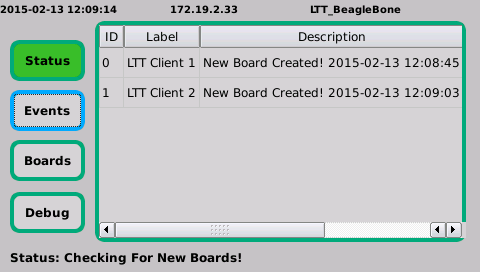
\includegraphics[width=0.5\textwidth ]{img/GUI/Server_GUI_Events1.png}
\caption{Mess-Server GUI: Events Tab}
\label{figure_MessServerGUIEvents}
\end{center}
\end{figure}

Im Events Tab werden wichtige Ereignisse dargestellt. 

\textbf{Boards Tab}

\begin{figure}[H]
\begin{center}
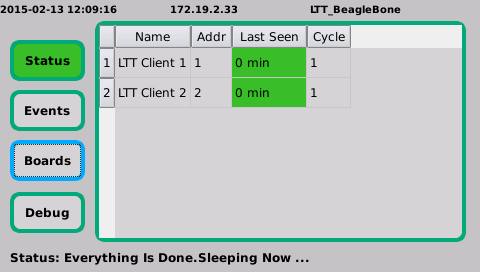
\includegraphics[width=0.5\textwidth ]{img/GUI/Server_GUI_Boards1.png}
\caption{Mess-Server GUI: Boards Tab}
\label{figure_MessServerGUIBoards}
\end{center}
\end{figure}

Das Boards Tab zeigt die derzeit aktiven Mess-Clients in einer Liste an. Als aktiv werden Mess-Clients bezeichnet, die mit einer gültigen Adresse in der Datenbank eingetragen sind. Angezeigt werden der Name, die Adresse, die vergangene Zeit seit dem es das letzten mal erfolgreich kontaktiert wurde und die Anzahl der erfolgreichen aufgenommenen Messzyklen.

\textbf{Debug Tab}

\begin{figure}[H]
\begin{center}
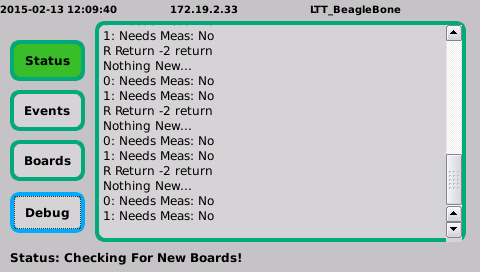
\includegraphics[width=0.5\textwidth ]{img/GUI/Server_GUI_Debug2.png}
\caption{Mess-Server GUI: Debug Tab}
\label{figure_MessServerGUIDebug}
\end{center}
\end{figure}

Der Zweck des Debug Tabs ist es die im Programmcode erzeugten Nachrichten anzuzeigen. Somit soll es möglich sein Fehler einfacher zu erkennen.

\subsubsection{RS232 Kommunikation}
Die RS232 Schnittstelle wird ausschließlich zur Kommunikation mit den Mess-Clients verwendet. Um die Erfolgschancen der Anfragen zu erhöhen, werden Fehlschläge erkannt und durch den Versuch des erneuten Sendens minimiert. Zwischen jedem Sendeversuch befindet sich eine kurze Verzögerung.
 

\subsubsection{Ethernet Kommunikation}

Um auf Netzwerkanfragen reagieren zu können, ist sowohl ein UDP-Server für Broadcast-Nachrichten als auch ein TCP-Server für die direkte Kommunikation realisiert.\\
Der UDP-Server dient dabei zur dynamischen Erkennung im Netzwerk. Dabei antwortet der Mess-Server auf Broadcast-Nachrichten mit seiner IP-Adresse und seinem Namen. Dies ermöglicht die einfache Eingliederung der Mess-Server in ein Netzwerk.
Der TCP-Server nimmt RS232- und SQL-Befehle an und leitet diese weiter. Dies ermöglicht den Fernzugriff auf die einzelnen Mess-Clients über ein Netzwerk. 

\begin{table}[H]
\begin{center}
\begin{tabularx}{\textwidth}{|c|c|c|X|}\hline 
 Command & Typ & Daten & Kommentar \\ \hline
 BeagleSendYourIP & UDP & - & Das BeagleBone antwortet dem Sender mit seiner IP Adresse und seinem Namen  \\ \hline
 BeagleUpdateConfig & UDP & - & Das BeagleBone aktualisiert seine Konfiguration aus der Config-Datei \\ \hline
 RS232CMD: & TCP & RS232 Rahmen & Das BeagleBone sende den empfangenen Rahmen über seine RS232 Schnittstelle \\ \hline
 SQLCMD: & TCP & SQL Anfrage & Das BeagleBone führt die SQL Anfrage aus \\ \hline
\end{tabularx}
\caption{Ethernet Befehlsliste}
\label{table_EthernetCommands}
\end{center}
\end{table}

\subsubsection{Webzugriff}

Um eine Übersicht über die gesammelten Daten auf einem Mess-Server zu erhalten, ist ein lighttpd Webserver installiert.



\newpage
\section{RS232 Protokoll}
\label{section_RS232_Protokoll}
Das Protokoll für die Kommunikation über die RS232 Schnittstelle dient zum Austausch von Informationen innerhalb des Systems zwischen den Akteuren. \\

Folgende Kriterien sollen dabei erfüllt werden:
\begin{itemize}
\item Adressierung individueller Kommunikationspartner
\item Senden verschiedener Befehle
\item Variable Größe der Daten
\item Sicherstellung der Validität der Übertragung
\item Erweiterbar
\end{itemize}



Um eine hohe Zuverlässigkeit gewährleisten zu können, wird eine geringe Bautrate von 2400 verwendet. Da nur geringe Datenmengen in großen Abständen auftreten, vermindert dass die Anfälligkeit der Übertragung gegenüber äußeren Einflüssen ohne dabei die Performance merkbar zu beeinflussen.\\
Des Weiteren wird ein Paritätsbit für eine Paritätsprüfung eingesetzt. Dieses Bit gibt an, ob die Anzahl der Einsen des Datenblocks gerade oder ungerade ist. Der Wert verwendeten Even-Paritätsbit ist 1, wenn die Summe der Einsen gerade ist und 0 wenn sie ungerade ist. Dadurch können grobe Fehler bei der Übertragung ausgemacht und korrigiert werden.
\newpage
\subsection{Aufbau}
\begin{table}[H]
\begin{center}
\begin{tabularx}{\textwidth}{|c|c|c|c|X|X|}\hline
 1. Byte & 2. Byte & 3. Byte & 4. Byte & 5. Byte und folgend & Letztes Byte\\ \hline
  Adresse \& R/W & Länge & Befehl & Unterbefehl & Nutzdaten & Checksumme\\ \hline
\end{tabularx}
\caption{Übertragungsrahmen}
\label{table_Frame}
\end{center}
\end{table}

Ein Rahmen des Protokolls besteht aus 4 Steuerbytes, 1 Checksummenbyte und maximal 30 Bytes an Nutzdaten. Durch diesen Aufbau können die Anforderungen erfüllt werden. Im folgenden Abschnitt wird auf die Zusammensetzung und die Funktion der einzelnen Bytes eingegangen.\\




\textbf{1. Byte: Adresse \& Read/Write}

\begin{table}[H]
\begin{center}
\begin{tabularx}{\textwidth}{|X|X|X|X|X|X|X|X|}\hline
 7. Bit & 6. Bit & 5. Bit & 4. Bit & 3. Bit & 2. Bit & 1. Bit & 0. Bit\\ \hline
 R/W & Addr6 & Addr5 & Addr4 & Addr3 & Addr2 & Addr1 & Addr0\\ \hline
\end{tabularx}
\caption{1. Byte: Adresse \& Read/Write}
\label{table_1Byte}
\end{center}
\end{table}

Das erste Byte des Übertragungsrahmens setzt sich aus 7 Adressbits und einem Lese-/Schreibbit zusammen. Die ersten 7 Bit (Addr0 - Addr6) bilden die Adresse des anzusteuernden Empfänger. Daraus ergibt sich ein Adressraum von möglichen 128 Adressen, wobei Adresse 0 für neue Mess-Clients zur einmaligen Anmeldung im System reserviert ist (siehe Abschnitt \ref{section_messclientverwaltung}).\\
Das höchste Bit ist das Lese-/Schreibbit. Mithilfe dieses Bits wird unterschieden, ob ein Befehl als Lese- oder Schreibzugriff interpretiert werden soll.\\

\begin{table}[H]
\begin{center}
\begin{tabular}{|l|l|}\hline
 R/W Bit & Beschreibung \\ \hline
 0 & Die Sender möchte lesen \\ \hline
 1 & Die Sender möchte schreiben \\ \hline
\end{tabular}
\caption{Read/Write}
\label{table_RW}
\end{center}
\end{table}

Ein Lesezugriff stellen dabei Anfragen dar. Dass heißt, dass keine Nutzdaten übertragen werden und eine Antwort des Empfängers mit den angeforderten Daten erwartet wird. Bei einem Schreibzugriff hingegen, werden immer Nutzdaten übertragen.\\

\newpage

\textbf{2. Byte: Rahmenlänge}

\begin{table}[H]
\begin{center}
\begin{tabularx}{\textwidth}{|X|X|X|X|X|X|X|X|}\hline
 7. Bit & 6. Bit & 5. Bit & 4. Bit & 3. Bit & 2. Bit & 1. Bit & 0. Bit\\ \hline
 Len7 & Len6 & Len5 & Len4 & Len3 & Len2 & Len1 & Len0\\ \hline
\end{tabularx}
\caption{2. Byte: Rahmenlänge}
\label{table_2Byte}
\end{center}
\end{table}

Das zweite Byte gibt die Länge des gesamten Rahmens inklusive Steuerbytes, Nutzdaten und Checksumme an. Die minimale Rahmenlänge beträgt 5 Byte. Dabei handelt es sich um eine Übertragung ohne Nutzdaten und es werden lediglich die 4 Steuerbytes und das Byte für die Checksumme übertragen. Dies geschieht beispielsweise bei einer Leseanfrage.\\
Die maximale Rahmenlänge beträgt 35 Byte. Hierbei werden zusätzlich zu den 4 Steuerbytes und dem Byte für die Checksumme auch die maximale Nutzlast von 30 Byte übertragen. Dieser Fall kann beispielsweise bei Schreibzugriffen auftreten.\\
Anhand der Länge kann eine erste Prüfung der Validität eines Rahmens durchgeführt werden. Sollte die Zahl der empfangenen Bytes sich von der Rahmenlänge unterscheiden, kann von einem ungültigen Rahmen ausgegangen werden.\\



\textbf{3. Byte: Befehl}

\begin{table}[H]
\begin{center}
\begin{tabularx}{\textwidth}{|X|X|X|X|X|X|X|X|}\hline
 7. Bit & 6. Bit & 5. Bit & 4. Bit & 3. Bit & 2. Bit & 1. Bit & 0. Bit\\ \hline
 Cmd7 & Cmd6 & Cmd5 & Cmd4 & Cmd3 & Cmd2 & Cmd1 & Cmd0\\ \hline
\end{tabularx}
\caption{3. Byte: Befehl}
\label{table_3Byte}
\end{center}
\end{table}

Das dritte Byte repräsentiert den Befehl. Dieser gibt an, welche Aktion ausgeführt oder welcher Parameter angesprochen wird. Da insgesamt ein Byte für den Befehl zur Verfügung steht, sind bis zu 256 unterschiedliche Befehle möglich.\\

\newpage

\textbf{4. Byte: Unterbefehl}

\begin{table}[H]
\begin{center}
\begin{tabularx}{\textwidth}{|X|X|X|X|X|X|X|X|}\hline
 7. Bit & 6. Bit & 5. Bit & 4. Bit & 3. Bit & 2. Bit & 1. Bit & 0. Bit\\ \hline
 Scmd7 & Scmd6 & Scmd5 & Scmd4 & Scmd3 & Scmd2 & Scmd1 & Scmd0\\ \hline
\end{tabularx}
\caption{4. Byte: Unterbefehl}
\label{table_4Byte}
\end{center}
\end{table}

Das vierte Byte ist der Unterbefehl. Damit ist es möglich einen Befehl genauer zu spezifizieren. So kann beispielsweise der Befehl zum Auslesen eines \ac{ADC} Wertes durch den Unterbefehl genau auf einen von 64 \acp{ADC} präzisiert werden. Im späteren Verlauf wird in Abschnitt \ref{section_BefehleUnterbefehle} näher auf die vorhandenen Befehle und Unterbefehle eingegangen.\\



\textbf{5. Byte und folgend: Nutzdaten}

\begin{table}[H]
\begin{center}
\begin{tabularx}{\textwidth}{|X|X|X|X|X|X|X|X|}\hline
 7. Bit & 6. Bit & 5. Bit & 4. Bit & 3. Bit & 2. Bit & 1. Bit & 0. Bit\\ \hline
 Data7 & Data6 & Data5 & Data4 & Data3 & Data2 & Data1 & Data0\\ \hline
\end{tabularx}
\caption{5. Byte und folgend: Nutzdaten}
\label{table_5Byte}
\end{center}
\end{table}

Das fünfte Byte und die darauf folgenden, tragen die Nutzdaten des Rahmens. Die Größe der Nutzdaten ist variable und lässt dich auf der Rahmenlänge ableiten. Bei zwei Byte Daten wird immer das höhere Byte zuerst übertragen.\\


\newpage

\textbf{Letztes Byte: Checksumme}

\begin{table}[H]
\begin{center}
\begin{tabularx}{\textwidth}{|X|X|X|X|X|X|X|X|}\hline
 7. Bit & 6. Bit & 5. Bit & 4. Bit & 3. Bit & 2. Bit & 1. Bit & 0. Bit\\ \hline
 CKS7 & CKS6 & CKS5 & CKS4 & CKS3 & CKS2 & CKS1 & CKS0\\ \hline
\end{tabularx}
\caption{Letztes Byte: Checksumme}
\label{table_LastByte}
\end{center}
\end{table}

Das letzte Byte ist immer die Checksumme um sicherzustellen, dass alle Daten komplett und fehlerfrei übertragen wurden.\\
Der Sender bildet dabei die Checksumme mittels einer XOR Verknüpfung aller Bytes eines Übertragungsrahmens. Beim Empfänger werden alle Bytes inklusive Checksumme erneut mit XOR Verknüpft, wobei ohne Fehler immer 0 das Ergebnis sein muss.\\


\textbf{Beispiel}

Sender:
 
Es wird angenommen das folgender Rahmen übertragen wird.
\begin{center}
\begin{tabular}{|c|c|c|c|}\hline
  Adresse & Länge & Befehl & Unterbefehl \\ \hline
  1 & 5 & 9 & 0 \\ \hline
\end{tabular}
\end{center}
Aus dem Rahmen wird dann mittels XOR die Checksumme gebildet.

\begin{center}
{\Large$1 \oplus 4 \oplus 9 \oplus 0 = 13$}\\
\end{center}

Anschließend wird die Checksumme als letztes Byte an den Rahmen an gehangen.
\begin{center}
\begin{tabular}{|c|c|c|c|c|}\hline
  Adresse & Länge & Befehl & Unterbefehl & Checksumme \\ \hline
  1 & 5 & 9 & 0 & 13 \\ \hline
\end{tabular}
\end{center}

Empfänger:

Sobald der Empfänger den rahmen erhält, verknüpft er alle Bytes erneut mittels XOR um die Gültigkeit zu prüfen.

\begin{center}
{\Large $1 \oplus 4 \oplus 9 \oplus 0 \oplus 13 = 0$}\\
\end{center}

Das Ergebnis 0 repräsentiert einen gültigen Rahmen und die Checksummenprüfung war erfolgreich.


\subsection{Befehle und Unterbefehle}
\label{section_BefehleUnterbefehle}
Für die Funktion des Systems sind verschiedene Befehle notwendig. Sie dienen zu Kommunikation zwischen den Akteuren.
Eine Übersicht über die implementierten Befehle der RS232 Schnittstelle findet sich in Tabelle \ref{table_RS232Commands}.\\

\begin{table}[H]
\begin{center}
\begin{tabularx}{\textwidth}{|X|c|X|c|}\hline 
 Befehl & Code & Unterbefehl & Datenbytes \\ \hline \hline
 ADC-Value & 0x00 & MUX-Kanal (0..63) & 2  \\ \hline
 Number Of Pulses & 0x04 & - & 1  \\ \hline
 Pulsewidth and -period & 0x05 & Pulsnummer (1..20) & 4  \\ \hline
 Perform Pulseupdate & 0x06 & - & 0   \\ \hline
 DAC-Value & 0x07 & - & 2 \\ \hline
 Temperature & 0x08 & - & 1  \\ \hline
 LTT Name & 0x09 & - & 1..30  \\ \hline
 Rs232-Address & 0x0A & - & 1 \\ \hline
 Measurement Intervall & 0x0C & Intervallnummer (0..2) & 4 \\ \hline
\end{tabularx}
\caption{RS232 Befehlsliste}
\label{table_RS232Commands}
\end{center}
\end{table}

\textbf{ADC-Value}\\
Der Befehl liest den Messwert eines Sensors des Mess-Clients. Mit dem Unterbefehl muss einer der 64 Sensoren spezifiziert werden. Die Datenmenge beträgt 2 Byte.\ 

\textbf{Number Of Pulses}\\
Dieser Befehl liest oder schreibt die Anzahl der Impulse im Pulsmuster des Mess-Clients. Die maximale Anzahl ist 20.\ 

\textbf{Pulsewidth and -period}\\
Ändert ein Pulsbreiten-/Pulsperiodenpaar. Der Unterbefehl bestimmt die Position im Pulsmuster.\ 

\textbf{DAC-Value}\\
Ließt oder schreibt den Wert für die Vorverstärkung zur Ansteuerung der Prüfobjekte.\ 

\textbf{Temperatur}\\
Der Befehl ließt den Wert des Temperatursensors.\ 

\textbf{LTT Name}\\
Ließt oder schreibt des Namen des Kommunikationspartners.\ 

\textbf{RS232-Adresse}\\
Ließt oder schreibt die Adresse für die Rs232 Kommunikation des Kommunikationspartners.\ 

\textbf{Measurement Intervall}\\
Ließt oder schreibt die Konfiguration der Messintervalle. Der Unterbefehl gibt dabei den Zeitraum (1 bis 3) an.\ 



